\section{Date: 2024-09-20}
\noindent \textbf{Series ID: G17MVSFLTRUCKS} 

\noindent This series is titled Regular Seasonal Factors: Light Truck Production and has a frequency of Monthly. The units are Seasonal Factor and the seasonal adjustment is Not Seasonally Adjusted.The observation start date is 1996-01-01 and the observation end date is 2025-06-01.The popularity of this series is 1. \\ 

\noindent \textbf{Series ID: PRGONUPIHCSA} 

\noindent This series is titled Medical Services Expenditures by Provider: Nursing Homes: Proprietary and Government Nursing Homes Price Index and has a frequency of Annual. The units are Index 2017=100 and the seasonal adjustment is Not Seasonally Adjusted.The observation start date is 2000-01-01 and the observation end date is 2021-01-01.The popularity of this series is 1. \\ 

\subsection{Regression Table}
\begin{center}
\begin{tabular}{lclc}
\toprule
\textbf{Dep. Variable:}              & value\_fred\_PRGONUPIHCSA & \textbf{  R-squared:         } &     0.002   \\
\textbf{Model:}                      &            OLS            & \textbf{  Adj. R-squared:    } &    -0.048   \\
\textbf{Method:}                     &       Least Squares       & \textbf{  F-statistic:       } &   0.04325   \\
\textbf{Date:}                       &      Fri, 20 Sep 2024     & \textbf{  Prob (F-statistic):} &    0.837    \\
\textbf{Time:}                       &          09:34:15         & \textbf{  Log-Likelihood:    } &   -90.742   \\
\textbf{No. Observations:}           &               22          & \textbf{  AIC:               } &     185.5   \\
\textbf{Df Residuals:}               &               20          & \textbf{  BIC:               } &     187.7   \\
\textbf{Df Model:}                   &                1          & \textbf{                     } &             \\
\textbf{Covariance Type:}            &         nonrobust         & \textbf{                     } &             \\
\bottomrule
\end{tabular}
\begin{tabular}{lcccccc}
                                     & \textbf{coef} & \textbf{std err} & \textbf{t} & \textbf{P$> |$t$|$} & \textbf{[0.025} & \textbf{0.975]}  \\
\midrule
\textbf{const}                       &      70.0979  &       81.638     &     0.859  &         0.401        &     -100.195    &      240.391     \\
\textbf{value\_fred\_G17MVSFLTRUCKS} &       0.1781  &        0.856     &     0.208  &         0.837        &       -1.608    &        1.964     \\
\bottomrule
\end{tabular}
\begin{tabular}{lclc}
\textbf{Omnibus:}       &  0.976 & \textbf{  Durbin-Watson:     } &    0.034  \\
\textbf{Prob(Omnibus):} &  0.614 & \textbf{  Jarque-Bera (JB):  } &    0.765  \\
\textbf{Skew:}          & -0.048 & \textbf{  Prob(JB):          } &    0.682  \\
\textbf{Kurtosis:}      &  2.091 & \textbf{  Cond. No.          } & 2.33e+03  \\
\bottomrule
\end{tabular}
%\caption{OLS Regression Results}
\end{center}

Notes: \newline
 [1] Standard Errors assume that the covariance matrix of the errors is correctly specified. \newline
 [2] The condition number is large, 2.33e+03. This might indicate that there are \newline
 strong multicollinearity or other numerical problems.

\subsection{Regression Plot}
\begin{figure}
\centering
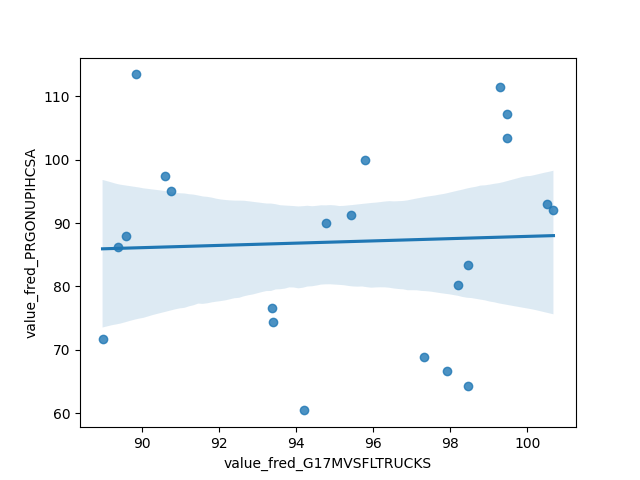
\includegraphics[scale = 0.9]{plots/plot_2024-09-20.png}
\caption{Regression Plot for 2024-09-20}
\end{figure}
\newpage
